\documentclass[12pt]{ctexart}
\usepackage{amsfonts,amssymb,amsmath,amsthm,geometry,enumerate,tikz,pgfplots}
\usepackage[colorlinks,linkcolor=blue,anchorcolor=blue,citecolor=green]{hyperref}
%introduce theorem environment
\theoremstyle{definition}
\newtheorem{definition}{定义}
\newtheorem{theorem}{定理}
\newtheorem{lemma}{引理}
\newtheorem{corollary}{推论}
\newtheorem{property}{性质}
\newtheorem{example}{例}
\theoremstyle{plain}
\newtheorem*{solution}{解}
\newtheorem*{remark}{注}
\geometry{a4paper,scale=0.8}

%article info
\title{\vspace{-2em}\textbf{连通性}\vspace{-2em}}
\date{ }
\begin{document}
	\maketitle
	\begin{definition}[连通性]
		设$X$为拓扑空间,若对任意非空集合$A$,$B$满足$A\cup B=X$,有$A\cap\overline{B}\neq\varnothing$或$\overline{A}\cap B\neq\varnothing$,则称$X$是\textbf{连通的}.
	\end{definition}
	\begin{theorem}
		实数轴是连通空间.
	\end{theorem}
	\begin{proof}
		设$\mathbb{R}=A\cup B$且$A\cap B=\varnothing$. 存在$a\in A$,$b\in B$,不失一般性,设$X=\{a\in A:a<b\}$,令$s=\sup X$.
		
		若$s\in X$,则对任意$s<x<b$,$x\notin A$,则$x\in B$,对任意$\varepsilon>0$,都有$x\in(s,b)$使得$|x-s|<\varepsilon$,故$s$是$B$的极限点,$s\in\overline{B}$,于是$A\cap\overline{B}\neq\varepsilon$.
		
		若$s\notin X$,则对任意小的$\varepsilon>0$,都有$a\in A$使得$a>s-\varepsilon$,则$s$是$A$的极限点,故$\overline{A}\cap B\neq\varnothing$.
	\end{proof}
	\begin{theorem}\label{itvconnect}
		实数轴的非空子集是连通的当且仅当这个子集是区间.
	\end{theorem}
	\begin{proof}
		区间的连通性是平凡的. 下面假设$X\subset\mathbb{R}$不是区间,则存在$a,b\in X$,$p\notin X$满足$a<p<b$,设$A=\{a\in X:a<p\}$,$B=X\backslash A=\{b\in X:b>p\}$,则$A\cap\overline{B}=\overline{A}\cap B=\varnothing$,推出$X$是不连通的. 于是实数轴的连通非空子集是区间.
	\end{proof}
	连通性也可以由其他命题刻画,有以下定理.
	\begin{theorem}
		下列命题是等价的.
		\begin{enumerate}
			\item $X$是连通的;
			\item $X$的既开又闭的子集只有$X$和$\varnothing$;
			\item $X$不能表示成两个非空不交开集的并;
			\item 不存在从$X$到多于一个点的离散空间的连续满射.
		\end{enumerate}
	\end{theorem}
	\begin{proof}
		1$\to$ 2 : 假设既开又闭的$A\subset X$,则$B=X\backslash A$也是既开又闭的. 于是$\overline{A}=A$,$\overline{B}=B$,
		$$A\cap\overline{B}=\overline{A}\cap B=A\cap B=\varnothing,$$
		而$X$是连通的,所以$A$和$B$必有一者为空集,另一者为$X$.
		
		2$\to$ 3 : 假设$X=U\cup V$,$U,\ V$是开集且$U\cap V=\varnothing$. 则$U=X\backslash V,\ V=X\backslash U$,开集的补集是闭的,于是$U,\ V$是既开又闭的,所以$U$和$V$必有一者为空集.
		
		3$\to$ 4 : 假设离散空间中存在两个点$a$,$b$,则$f^{-1}(a)\cup f^{-1}(b)=X$,$f^{-1}(a)\cap f^{-1}(b)=\varnothing$,且$f^{-1}(a)$和$f^{-1}(b)$都是非空开集,这与3矛盾.
		
		4$\to$ 1 : 如果$X$是不连通的,则存在$A\cup B=X$使得$A\cap\overline{B}=\overline{A}\cap B=A\cap B=\varnothing$,注意到$A$,$B$是不交开集. 于是令
		\begin{equation*}
			f=\left\{
			\begin{aligned}
				&1,\ x\in A,\\
				&-1,\ x\in B,
			\end{aligned}
			\right.
		\end{equation*}
		则$f$是从$X$到$\{1,-1\}$的连续满射. 由逆否命题的等价性得证.
	\end{proof}
	可以发现,空集$\varnothing$也符合命题2,于是约定空集也是连通的.
	\begin{theorem}
		连通空间在连续映射下的像是连通的.
	\end{theorem}
	\begin{proof}
		设$f:X\to Y$是连续满射,且$X$是连通的. 设任意$A\subset Y$既开又闭,则$f^{-1}(A)$既开又闭,由于$X$的连通性,$f^{-1}(A)=\varnothing$或$X$,于是$A=\varnothing$或$Y$,则$Y$是连通的.
	\end{proof}
	\begin{corollary}
		若$X$和$Y$同胚,则$X$连通当且仅当$Y$连通.
	\end{corollary}
	\begin{example}
		利用连通性证明介值定理.
	\end{example}
	\begin{proof}
		设连续函数$f:\left[a,b\right]\to\mathbb{R}$,$f(a)<0$,$f(b)>0$,则由定理\ref{itvconnect}得,$\left[a,b\right]$是连通的,$\mathrm{Im}(\left[a,b\right])$是连通的,于是$\left[f(a),f(b)\right]$是区间,故存在$c\in\left[a,b\right]$使得$f(c)=0$.
	\end{proof}
	\begin{theorem}
		令$X$为拓扑空间,若$Z\subset X$是连通的,且$Z$在$X$中稠密,则$X$是连通的.
	\end{theorem}
	\begin{proof}
		设$A\subset X$既开又闭,由于$Z$是稠密的,于是$A\cap Z\neq\varnothing$,于是$A\cap Z\subset Z$是既开又闭的,$Z$是连通的,于是$A\cap Z=Z$,于是$Z\subset A$,于是
		$X=\overline{Z}\subset\overline{A}=A\subset X$,故$A=X$,$X$是连通的.
	\end{proof}
	\begin{corollary}
		若$Z$是$X$的连通子空间,对于$Y$满足$Z\subset Y\subset\overline{Z}$,则$Y$是连通的. 特别地,$\overline{Z}$也是连通的.
	\end{corollary}
	\begin{proof}
		$Z$在$Y$中的闭包为$\overline{Z}\cap Y=Y$,则$Z$在$Y$中稠密,于是$Y$是连通的.
	\end{proof}
	\begin{theorem}\label{kebab}
		设$\mathcal{F}=\{M_i:\bigcup_{i\in I} M_i=X\}$是$X$的若干子集组成的集合,若$M_i$都是连通的,且$\overline{M_i}\cap \overline{M_j}\neq\varnothing,\ i,j\in I$,则$X$是连通的.
	\end{theorem}
	\begin{proof}
		设$A\subset X$既开又闭,则对任意$M_i\in\mathcal{F}$,$A\cap M_i$也是既开又闭的. 对任意$M_i$,若$A\cap M_i=\varnothing$,则$A\cap\left(\bigcup_{i\in I}M_i\right)=A\cap X=\varnothing$,$A=\varnothing$. 
		
		若对某些$M_i$,$A\cap M_i\neq\varnothing$既开又闭,且$M_i$为连通的,于是$A\cap M_i=M_i$,$M_i\subset A$,$\overline{M_i}\subset\overline{A}$.
		
		假设存在$M_j$,使得$A\cap M_j=\varnothing$,则$M_j\subset X\backslash A$,于是$\overline{M_j}\subset\overline{X\backslash A}=X\backslash A=X\backslash\overline{A}$.
		
		而$\overline{A}\cup\left(X\backslash\overline{A}\right)=\varnothing$,于是$\overline{M_i}\cap\overline{M_j}=\varnothing$与题意不符. 于是对所有的$M_i$,只要存在$M_{i_0}$使得$M_{i_0}\cap A\neq\varnothing$,则任意$M_i\in\mathcal{F}$,都有$M_i\cap A\neq\varnothing$,则$M_i\subset A$.故
		$$X=\bigcup_{i\in I}M_i\subset A\subset X,$$
		故$A=X$.
	\end{proof}
	\begin{definition}
		设$A,B\subset X$,若$\overline{A}\cap\overline{B}=\varnothing$,则称$A$和$B$是\textbf{相互隔离的}.
	\end{definition}
	\begin{theorem}
		若$X$和$Y$都是连通的,则$X\times Y$也连通.
	\end{theorem}
	\begin{proof}
		由于$\{x\}\times Y$与$Y$同胚,于是$\{x\}\times Y$是连通的. 同理,$X\times \{y\}$也是连通的,且与$\{x\}\times Y$交于$(x,y)$. 由定理\ref{kebab},$Z(x,y)=\left(\{x\}\times Y\right)\cup\left(X\times \{y\}\right)$也是连通的. 对任意$Z(x_1,y_1)$和$Z(x_2,y_2)$,$Z(x_1,y_1)\cap Z(x_2,y_2)=\{(x_1,y_2),(x_2,y_1)\}\neq\varnothing$,于是
		$$X\times Y=\bigcup_{x\in X, y\in Y}Z(x,y)$$
		是连通的.
	\end{proof}
	\begin{remark}
		若$X\times Y$非空,则由$X\times Y$连通可以推得$X$和$Y$都连通.
	\end{remark}
	若整个空间不是连通的,分为了若干相互分离的连通的部分,称为连通分支. 等价定义如下.
	\begin{definition}[连通分支]
		设$U$是$X$的连通子集,若$U$不是$X$的任一连通子集的真子集,则称为$X$的\textbf{连通分支}.
	\end{definition}
	\begin{theorem}
		拓扑空间的任一连通分支是闭集.
	\end{theorem}
	\begin{proof}
		若连通集$U\subset X$,则$\overline{U}$是连通的,且$U\subset\overline{U}$,若$U$不是闭集,则$U\subsetneqq\overline{U}$,于是$U$不是连通支集.
	\end{proof}
	\begin{theorem}
		拓扑空间的任意两个连通分支相互隔离.
	\end{theorem}
	\begin{proof}
		若连通分支$\overline{U}\cap \overline{V}\neq\varnothing$,由定理\ref{kebab},得$U\cup V$也是连通的,则$U$、$V$不再是极大连通子集,即连通分支.
	\end{proof}
	\begin{definition}[完全不连通]
		若拓扑空间$X$的每一点都是它的一个连通分支,则称$X$是\textbf{完全不连通}的.
	\end{definition}
	\begin{definition}[局部连通]
		设$X$为拓扑空间,若对任意$x\in X$,任意邻域$U\ni x$,都有连通的邻域$V$,使得$x\in V\subset U$,则称$X$是\textbf{局部连通的}.
	\end{definition}
	连通性的一个特例为道路连通性. 首先定义道路.
	\begin{definition}[道路]
		设$X$为拓扑空间,连续映射$\gamma:\left[0,1\right]\to X$,称$\gamma$为\textbf{道路}. $\gamma(0)$和$\gamma(1)$分别称为道路的\textbf{起点}和\textbf{终点}.
	\end{definition}
	\begin{definition}[道路连通]
		设$X$为拓扑空间,对任意$x_0,x_1\in X$,都存在$\gamma$使得$\gamma(0)=x_0,\gamma(1)=x_1$,则称$X$是\textbf{道路连通的}.
	\end{definition}
	\begin{theorem}
		设拓扑空间$X$和$Y$同胚,则$X$道路连通当且仅当$Y$道路连通.
	\end{theorem}
	\begin{proof}
		不妨设连续映射$f:X\to Y$,则$f^{-1}$也连续. 若$X$道路连通,有连续映射$\gamma:\left[0,1\right]\to X$,则$\gamma'=f\circ\gamma:\left[0,1\right]\to Y$是$Y$的道路,对任意$y_0,y_1$,都有$x_0,x_1$满足$f(x_0)=y_0$,$f(x_1)=y_1$,且有$\gamma(0)=x_0$,$\gamma(1)=x_1$,于是$\gamma'(0)=y_0$,$\gamma'(1)=y_1$,故$Y$道路连通. 同理可设$Y$道路连通,得到$X$道路连通.
	\end{proof}
	\begin{theorem}
		道路连通空间是连通的.
	\end{theorem}
	\begin{proof}
		设$X$是道路连通的,既开又闭的非空集合$A\subsetneqq X$,则对$x\in A$,$y\in X\backslash A$,存在从$x$到$y$的道路$\gamma$,则$\gamma^{-1}(A)\subsetneqq\left[0,1\right]$,而$\gamma^{-1}(A)$是既开又闭且非空的,且$\left[0,1\right]$是连通的,那么$\gamma^{-1}(A)=\left[0,1\right]$,矛盾!于是$A=X$,故$X$是连通的.
	\end{proof}
	设$\alpha$是从$x$到$y$的道路,$\beta$是从$y$到$z$的道路,则
	\begin{equation*}
		\gamma=\left\{
		\begin{aligned}
			&\alpha(2t),\qquad &0\leqslant t\leqslant\frac{1}{2}\\
			&\beta(2t-1),\qquad &\frac{1}{2}<t\leqslant 1
		\end{aligned}
		\right.
	\end{equation*}
	是从$x$到$z$的道路.
	\begin{theorem}
		Euclidean空间的连通开集是道路连通的.
	\end{theorem}
	\begin{proof}
		设$X\subset\mathbb{R}^n$是连通开集. 对任意$x\in X$,设$U(x)=\left\{y\in X|\text{存在从}x\text{到}y\text{的道路}\right\}$,则$U(x)$非空($x\in U(x)$),下证$U(x)=X$.
		
		设开球$B(y,\varepsilon)$,对$z\in B$,$y$到$z$的道路是一条直线,于是有从$x$到$z$的道路,故$z\in U(x)$,于是$B(y,\varepsilon)\subset U(x)$,$U(x)$是开集. 而$X\backslash U(x)=\bigcup\left\{U(y):y\in X\backslash U(x)\right\}$,且任意$U(y)$为开集,于是$X\backslash U(x)$为开集,$U(x)$为闭集. $U(x)$为既开又闭的非空集合,于是$U(x)=X$.
	\end{proof}
	道路连通空间是连通的,但连通空间不一定道路连通. 下面是一个连通但不道路连通的反例.
	\begin{example}
		定义
		$$Y=\left\{(0,y)\ |\ -1\leqslant y\leqslant 1\right\},$$
		$$Z=\left\{(x,\sin\frac{\pi}{x})\ | \ 0<x\leqslant 1\right\},$$
		则$X=Y\cup Z$是连通的,而不是道路连通的.
	\end{example}
	\begin{proof}
		$Z$是$\left(0,1\right]$上连续映射的像,因此$Z$连续. 而$Z$在$\mathbb{R}^2$的闭包是$X$,于是$X$是连通的.
		
		假设存在道路
		$$\gamma:\left[0,1\right]\to X,\quad \gamma(t)=(\gamma_1(t),\gamma_2(t))$$
		使得$\gamma(0)=(0,0)$,$\gamma(1)=(1,0)$. 令
		$$s=\sup\left\{t\ |\ \gamma_1(t)=0\right\},$$
		则$s<1$,$\gamma_1(s)=0$,且对任意$t>s$,有$\gamma_1(t)>0$. 于是对任意$t>s$,有
		$$\gamma_2(t)=\sin\frac{\pi}{\gamma_1(t)},$$
		于是由$\gamma_1$的连续性,存在递减数列$t_n\to s$使得$\gamma_1(t_n)=\frac{2}{2n+1}$. 则
		$$\gamma_2(t_n)=(-1)^n\nrightarrow \gamma_2(s),$$
		矛盾!
	\end{proof}
	\begin{figure}[htbp]
		\centering
		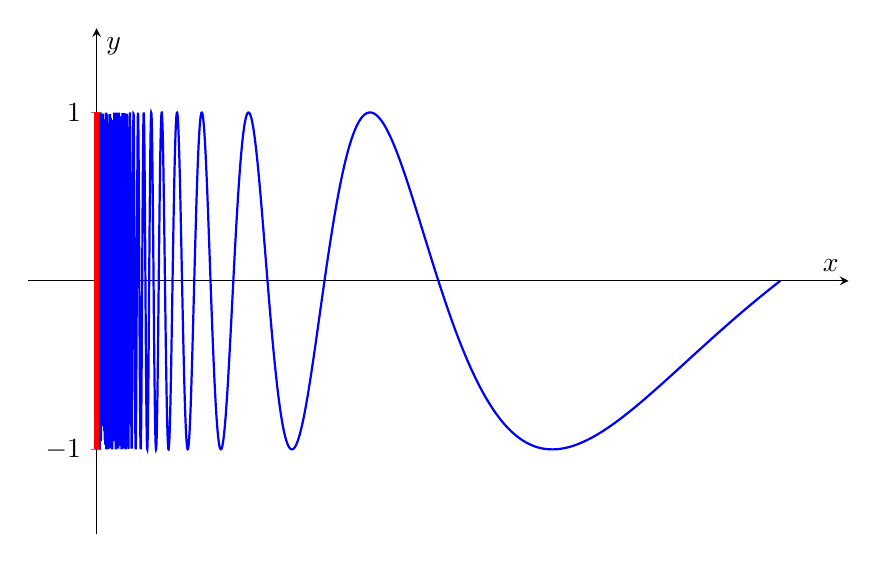
\begin{tikzpicture}
		\begin{axis}[
			width=12cm,
			height=8cm,
			xmin=-0.1, xmax=1.1,
			ymin=-1.5, ymax=1.5,
			axis lines=middle,
			xlabel=$x$,
			ylabel=$y$,
			xtick={0},
			ytick={-1,0,1},
			samples=5000, % 高采样率用于表现振荡
			clip=false,
			]
			
			% 绘制正弦曲线部分 S = {(x, sin(\pi/x)) | 0 < x ≤ 1}
			\addplot[domain=0.001:1, blue, thick] {sin(deg(pi/x))};
			
			% 绘制垂直线段 V = {(0,y) | -1 ≤ y ≤ 1}
			%\draw[ultra thick, red] (0,-1) -- (0,1);
			
			\pgfplotsextra{
				\draw[red,ultra thick] (axis cs:0,-1) -- (axis cs:0,1);
			}					
		\end{axis}
	\end{tikzpicture}
	
	\caption{拓扑学家的正弦曲线}
	\label{sin}
	\end{figure}
	与连通分支类似,定义道路连通分支.
	\begin{definition}[道路连通分支]
		设$U$是$X$的道路连通子集,若$U$不是$X$的任一道路连通子集的真子集,则称为$X$的\textbf{道路连通分支}.
	\end{definition}
	然而,对于道路连通分支没有相互分离的结论,而且也不一定是闭的. 例如图\ref{sin},$Y$和$Z$既不相互分离,$Z$也不是闭的.
	
	与局部连通类似,定义局部道路连通.
	\begin{definition}[局部道路连通]
		设$X$为拓扑空间,若对任意$x\in X$,任意邻域$U\ni x$,都有道路连通的邻域$V$,使得$x\in V\subset U$,则称$X$是\textbf{局部道路连通的}.
	\end{definition}
\end{document}